\documentclass{beamer}

\usepackage{graphicx}
\usepackage[absolute,overlay]{textpos}
\usepackage{listings}
\usepackage{color}
\usepackage{textcomp}
\usepackage[version=3]{mhchem}

\definecolor{listinggray}{gray}{0.9}
\definecolor{lbcolor}{rgb}{0.9,0.9,0.9}
\lstset{
	backgroundcolor=\color{lbcolor},
	tabsize=4,
	rulecolor=,
	language=matlab,
        basicstyle=\tiny,
        upquote=true,
%         aboveskip={1.5\baselineskip},
        columns=fixed,
        showstringspaces=false,
        extendedchars=true,
        breaklines=true,
        prebreak = \raisebox{0ex}[0ex][0ex]{\ensuremath{\hookleftarrow}},
        %frame=single,
        showtabs=false,
        showspaces=false,
        showstringspaces=false,
        identifierstyle=\ttfamily,
        keywordstyle=\color[rgb]{0,0,1},
        commentstyle=\color[rgb]{0.133,0.545,0.133},
        stringstyle=\color[rgb]{0.627,0.126,0.941},
}


% \usepackage{default}
\usetheme{Copenhagen}
\newcommand{\blankline}{\quad\pagebreak[2]}
\title{CLACINDIA Workshop \\
Lab Session\\
       Part 0: Computer Programming, why we need it?}
\author{Nikolay Koldunov}

\date{JNU\\
       2014}

\pgfdeclareimage[height=0.8cm]{logo}{logos.png}
\setlength{\TPHorizModule}{1mm}
\setlength{\TPVertModule}{1mm}
\newcommand{\MyLogo}{%
\begin{textblock}{14}(97.0,81.0)
  \pgfuseimage{logo}
\end{textblock}
}


\begin{document}


\begin{frame}
\titlepage
\MyLogo
\end{frame}

%%%%%%%%%%%%%%%%%%%%%%%%%%%%%%
%%%%%%%%%%%%%%%%%%%%%%%%%%%%%%%

\begin{frame}[fragile]
\frametitle{Definition}
\textbf{Computer programming} (often shortened to \textbf{programming} or \textbf{coding}) is the process of writing, testing, debugging, and maintaining the \textit{source code} of \textit{computer programs}. The purpose of programming is to create a program that exhibits a certain desired behaviour.
\end{frame}
%%%%%%%%%%%%%%%%%%%%%%%%%%%%%%
%%%%%%%%%%%%%%%%%%%%%%%%%%%%%%%

\section{Why we need programming?}

\begin{frame}
\frametitle{Why geoscientists need programming skills?}
\pause
\begin{itemize}
 \item To quickly obtain the data.
 \item Manipulations with huge amounts of data, extracting data that we need
 \item Data analysys. 
 \item Data vizualization.
 \item Presentation of the results (web, \LaTeX{})

\end{itemize}

\blankline

\begin{center}
We need programming to do it \textbf{efficienly}.\\
Science is developing very fast. There is no ``perfect'' software, that will do exactly what you need
\end{center}

\end{frame}

%%%%%%%%%%%%%%%%%%%%%%%%%%%%%%%%%%%%%%%%%%%
%%%%%%%%%%%%%%%%%%%%%%%%%%%%%%%%%%%%%%%%%%%

\begin{frame}[fragile]
\frametitle{Obtaining of data} 
\begin{center}
Download all data files from the ftp directory:\\ 
\end{center}



\begin{columns}[t]
\begin{column}{.5\textwidth}
``Simple'' way
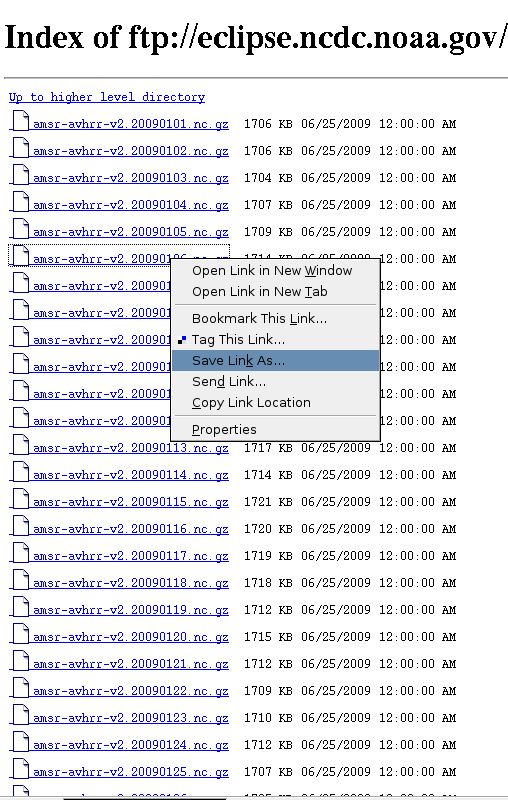
\includegraphics[width=0.6\textwidth,angle=00]{obt.png}
\vspace{3cm} 
\end{column}
\begin{column}{.5\textwidth}
``Difficult`` way
\begin{lstlisting}
ftp> mget * 
\end{lstlisting}
\end{column}
\end{columns}

\end{frame}

%%%%%%%%%%%%%%%%%%%%%%%%%%%%%%%%%%%%%%%%%%%%%%%%
%%%%%%%%%%%%%%%%%%%%%%%%%%%%%%%%%%%%%%%%%%%%%%%%%%
\begin{frame}[fragile]
\frametitle{Manipulations with data} 
\begin{center}
Open AARI sea ice data from nsidc.org:\\ \end{center}

\begin{columns}[t]
\begin{column}{.5\textwidth}
``Simple'' way


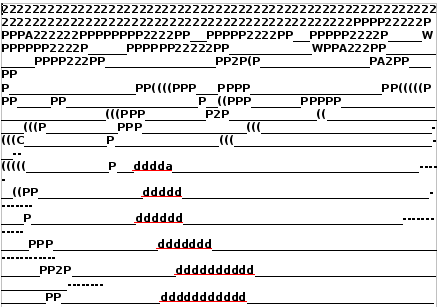
\includegraphics[width=0.8\textwidth,angle=00]{binSoffice.png}

\end{column}
\begin{column}{.5\textwidth}
``Difficult`` way

\begin{lstlisting}
file=fopen('E19750806.v0.bin','rb');
map=fread(file,[721,721],'uint8')
imagesc(map)
\end{lstlisting}
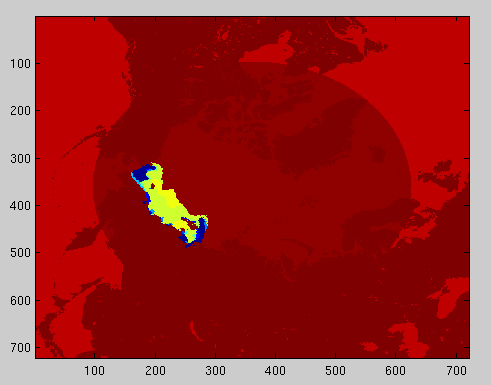
\includegraphics[width=\textwidth,angle=00]{matlabAARI.png}
\end{column}
\end{columns}

\end{frame}

%%%%%%%%%%%%%%%%%%%%%%%%%%%%%%%%%%%%%%%%%%%%%%%%%%%%%%%%%%%%%
%%%%%%%%%%%%%%%%%%%%%%%%%%%%%%%%%%%%%%%%%%%%%%%%%%%%%%%%%%%%%
\begin{frame}[fragile]
\frametitle{Data analysys} 
\begin{center}
Average of every second record :\\ \end{center}

\begin{columns}[t]
\begin{column}{.5\textwidth}
``Simple'' way


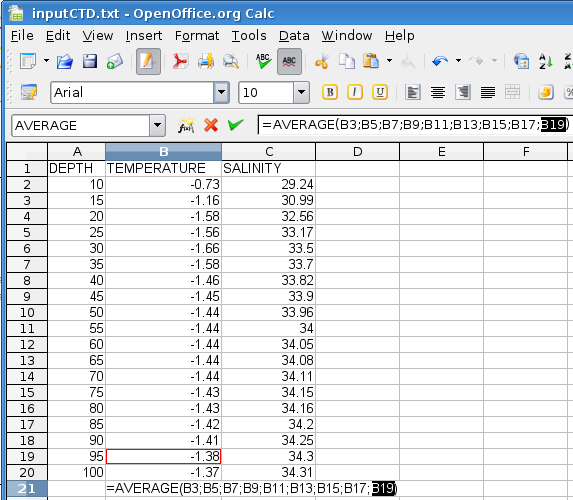
\includegraphics[width=0.9\textwidth,angle=00]{sprsh.png}

\end{column}
\begin{column}{.5\textwidth}
``Difficult`` way

\begin{lstlisting}
>> avrg = mean(temperature(2:2:end))

avrg =

   -1.4274
\end{lstlisting}
\end{column}
\end{columns}

\end{frame}
%%%%%%%%%%%%%%%%%%%%%%%%%%%%%%%%%%%%%%%%%%%%%%%
%%%%%%%%%%%%%%%%%%%%%%%%%%%%%%%%%%%%%%%%%%%%%%%
\begin{frame}[fragile]
\frametitle{Data visualization} 
\begin{center}
Plot Temperature vs Depth\\ \end{center}

\begin{columns}[t]
\begin{column}{.5\textwidth}
``Simple'' way


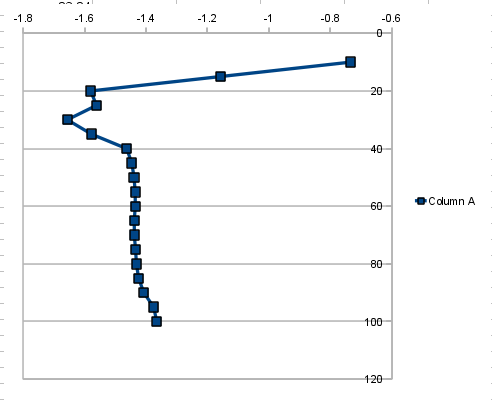
\includegraphics[width=0.8\textwidth,angle=00]{graphOO.png}

\end{column}
\begin{column}{.5\textwidth}
``Difficult`` way
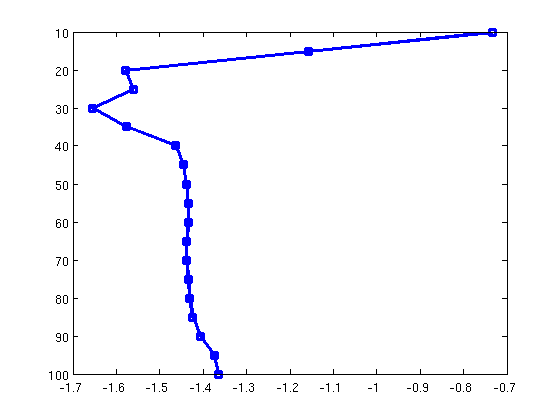
\includegraphics[width=0.8\textwidth,angle=00]{mat_graph.png}
\begin{lstlisting}
plot(temperature,depth,'-s')
set(gca,'ydir','reverse')
\end{lstlisting}
\end{column}
\end{columns}

\pause

\begin{center}
But what if you need 1000 plots?\end{center}
\end{frame}
%%%%%%%%%%%%%%%%%%%%%%%%%%%%%%%%%%%%%%%%%%%%%%%%%%%%%
%%%%%%%%%%%%%%%%%%%%%%%%%%%%%%%%%%%%%%%%%%%%%%%%%%%%%
\begin{frame}[fragile]
\frametitle{Data visualization} 

\begin{center}
IBCAO\\
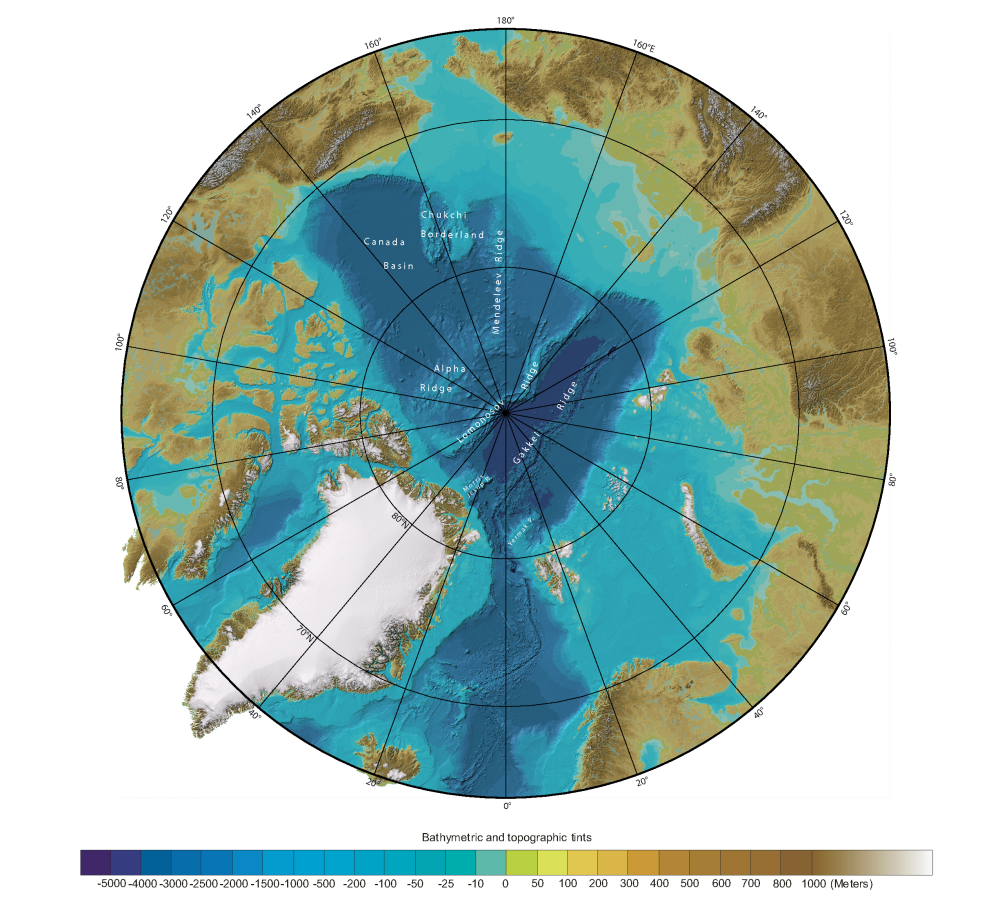
\includegraphics[width=0.7\textwidth,angle=00]{IBCAO.png}\end{center}

\end{frame}
%%%%%%%%%%%%%%%%%%%%%%%%%%%%%%%%%%%%%%%%%%%%%%%%
%%%%%%%%%%%%%%%%%%%%%%%%%%%%%%%%%%%%%%%%%%%%%%%%

\begin{frame}[fragile]
\frametitle{Data visualization} 
\begin{center}
GEBCO\\
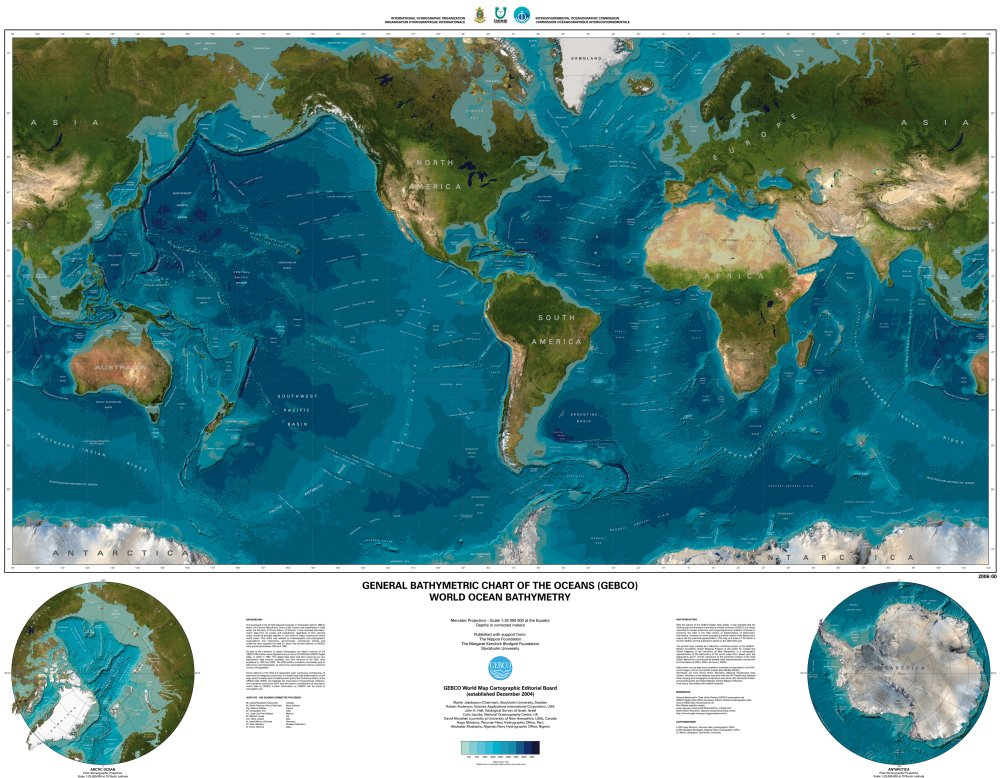
\includegraphics[width=0.8\textwidth,angle=00]{gda_world_map_small.jpg}\end{center}
\end{frame}
%%%%%%%%%%%%%%%%%%%%%%%%%%
%%%%%%%%%%%%%%%%%%%%%%%%



\begin{frame}[fragile]
\frametitle{Data visualization} 
\begin{center}
Create participants map\\ \end{center}

\begin{columns}[t]
\begin{column}{.5\textwidth}



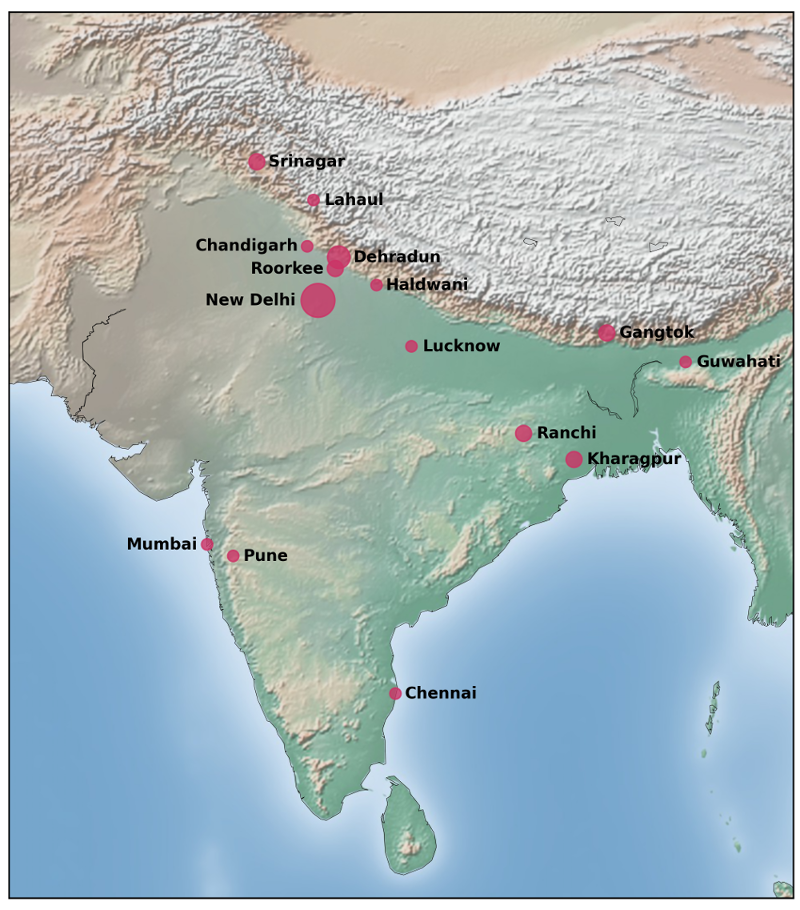
\includegraphics[width=1\textwidth,angle=00]{participants_map.png}

\end{column}
\begin{column}{.5\textwidth}
%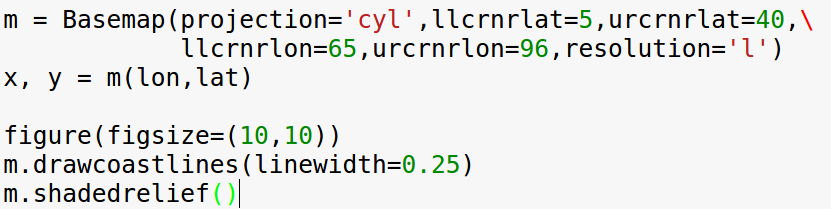
\includegraphics[width=0.8\textwidth,angle=00]{code_prt.png}
\begin{lstlisting}
m = Basemap(projection='cyl',llcrnrlat=5,urcrnrlat=40,\
            llcrnrlon=65,urcrnrlon=96,resolution='l')
x, y = m(lon,lat)

figure(figsize=(10,10))
m.drawcoastlines(linewidth=0.25)
m.shadedrelief()
\end{lstlisting}
\end{column}
\end{columns}
\end{frame}
%%%%%%%%%%%%%%%%%%%%%%%
%%%%%%%%%%%%%%%%%%%%%%%

\begin{frame}[fragile]
\frametitle{Presentation of results} 
\begin{center}
Web\\
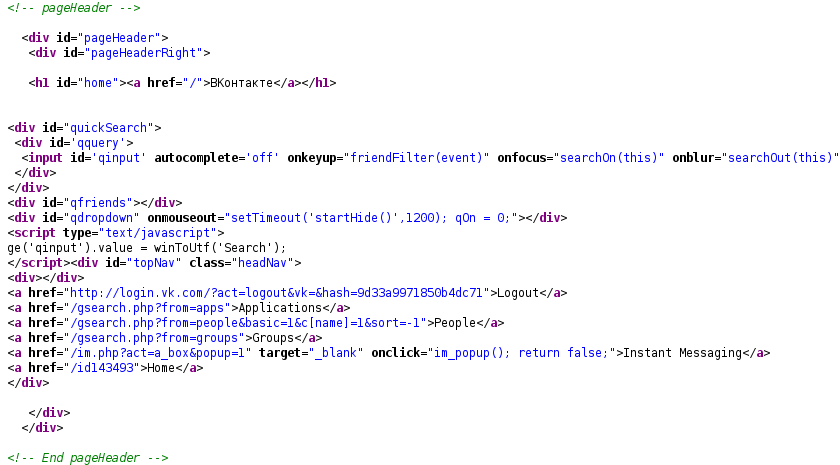
\includegraphics[width=0.7\textwidth,angle=00]{vkontakte1.png}\end{center}
\end{frame}
%%%%%%%%%%%%%%%%%%%%%%%%%%%%%%
%%%%%%%%%%%%%%%%%%%%%%%%%%%%%%%

\begin{frame}[fragile]
\frametitle{Presentation of results}
\begin{center}
\LaTeX{}\\
\begin{example}
\ce{Zn^2+
  <=>[\ce{+ 2OH-}][\ce{+ 2H+}]
  $\underset{\text{amphoteres Hydroxid}}{\ce{Zn(OH)2 v}}$
  <=>C[+2OH-][{+ 2H+}]
  $\underset{\text{Hydroxozikat}}{\cf{[Zn(OH)4]^2-}}$
}
\end{example}

\begin{example}
\begin{eqnarray}
B_g &=& \frac{1}{h}\left( \mathcal{B}_{in} - \int_{-h}^0B_{Ek}dz \right) \nonumber \\
&=& \frac{1}{h}\frac{g}{\rho_0}\left( \frac{\alpha Q_{net}}{C_w} - \rho_0 \beta S_{net}\right)
- \frac{1}{h}\int_{-h}^0
\frac{g}{\rho_0}\frac{1}{\rho f}\vec{k}\times \frac{\partial \tau}{\partial z} \cdot\nabla\sigma_m dz
\nonumber \\
&=& \frac{1}{h}\frac{g}{\rho_0}\left( \frac{\alpha Q_{net}}{C_w} - \rho_0 \beta S_{net}\right)
- \frac{g}{\rho_0}\frac{1}{\rho f \delta_e}\vec{k}\times\tau\cdot\nabla\sigma_m
\end{eqnarray} 
\end{example}

\end{center}
\end{frame}
%%%%%%%%%%%%%%%%%%%%%%%%%%%%%%
%%%%%%%%%%%%%%%%%%%%%%%%%%%%%%%

\begin{frame}[fragile]
\frametitle{You need it to get a job}
\begin{center}
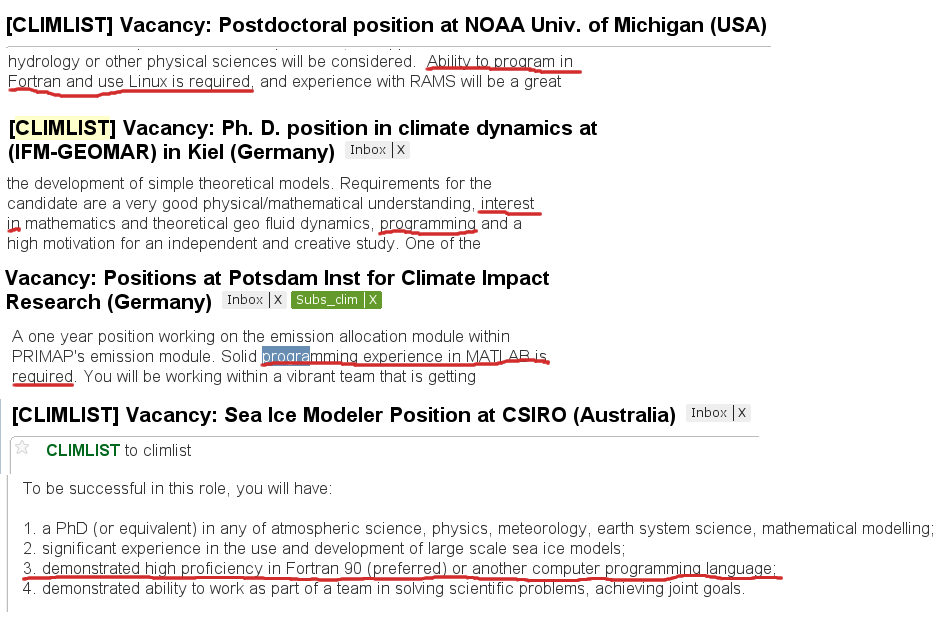
\includegraphics[width=0.8\textwidth,angle=00]{job.png}\end{center}
\end{frame}
%%%%%%%%%%%%%%%%%%%%%%%%%%%%%%
%%%%%%%%%%%%%%%%%%%%%%%%%%%%%%%



\begin{frame}[fragile]
\frametitle{You already have some programming skills}
\begin{center}
Calculate summ of 2 and 2 in Exel
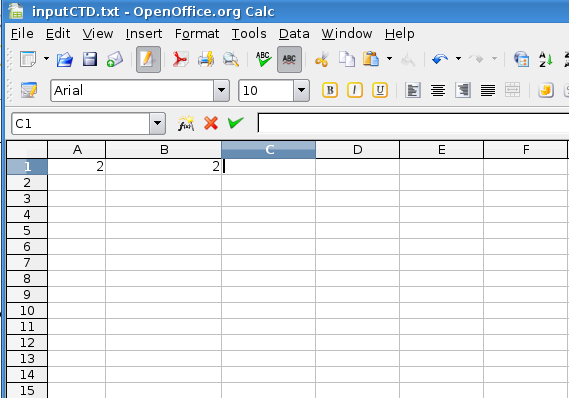
\includegraphics[width=0.8\textwidth,angle=00]{2x2.png}\end{center}
\end{frame}
%%%%%%%%%%%%%%%%%%%%%%%%%%%%%%
%%%%%%%%%%%%%%%%%%%%%%%%%%%%%%%
\begin{frame}[fragile]
  \frametitle{You already have some programming skills}
    \begin{block}{Here is the source code of your program:}

      A1+B1

    \end{block}
\blankline
    \begin{block}{When you press Enter the program is executed and print the result:}
      4
    \end{block}
\blankline
\blankline
\pause
Programs should be written in a programming language.

\end{frame}

% 
% \begin{frame}[fragile]
% \frametitle{Programming languages}
% \begin{block}
%   \begin{lstlisting}
%     #include <iostream.h>
%     main()
% 
%    \end{lstlisting}
% \end{block}
% 
% 
% 
% \end{frame}
%%%%%%%%%%%%%%%%%%%%%%%%%%%%%%
%%%%%%%%%%%%%%%%%%%%%%%%%%%%%%%

% %the "fragile" option is nessesary if you want to include listins  code
% \begin{frame}[fragile]
% \frametitle{code example} 
% 
% 
% \begin{lstlisting}
% if draw
%     print([outputpath, 'mygraph.eps'],'-depsc')
% end
% \end{lstlisting}
% 
% \begin{lstlisting}[language=Python]
% try:
%     file_name = sys.argv[1]
% except:
%     print "Usage:",sys.argv[0], "input_file "
%     sys.exit(1)
% \end{lstlisting}
% 
% 
% \end{frame}

\end{document}
